
\section{Six Key Words}
Satellite image, Lake size scaling, Fractal dimension, Machine learning, Carbon fluxes, Microbes. 
\section{Introduction}
The carbon flow is a crucial indicator for calculating the amount of carbon emissions. Several studies indicated that ponds and lakes, particularly those in forested areas or with thermokarst deposits in the Arctic or Tibet Plateau, are among those that produce the most carbon\citep{serikova2019high,holgerson2017gas,karlsson2021carbon}.A small pond would retain a lot of carbon and release it into the air, according to \cite{holgerson2016large}. As \cite{cael2016size} reported , both the local lake view and the global lake view show that the lake size does not scale according to the power law. The \cite{mandelbrot1982fractal} provided a fractal theory that scaled the ponds differently. Hence, \cite{cael2016size} study of the lakes in Sweden and the lakes across the world reveals a considerable relationship between lake density and area. When the lakes shrink in size, the difference becomes apparent. In addition, the shallow small ponds tend to release carbon by active microbes decomposing sediment and primary producer consuming\citep{bartosiewicz2015greenhouse,colina2022role}. Large lakes may cover broad surface area, but millions of smaller lakes with more active reactions would create and store more carbon than a single huge lake.
Thus, there is a trend to research tiny lakes across the world that emit carbon. In my proposal, the worldwide lake density with areas would first be restudied to more precisely confirm the findings in \cite{cael2016size} study. Then, the link between carbon emissions, microbial response, and tiny lake would then be examined.

\section{Proposed Methods}

1. Locate the river data from the global and regional lake census using the \cite{cael2016size} method. Then, in order to broaden the scope of my research, I will group various lakes according to latitude or continent. Then, test the global river's power law distribution and ordinary lease squares regression on the regional lakes. Moreover, compare them all at once. Apart from that, certain regions' lakes would be verified using free or paid high resolution satellite maps. last, the machine learning technique would aid in simulating any potential relationships that would fit more closely than the conventional least square method. R and HPC may collaborate to facilitate code execution.
\\
2. Apart from the restudying the scaling lakes problems.The rest time would be spent researching the connections between carbon emissions, microbial biomass, and small lakes. Data from a different research's study may be used to evaluate the association.

\section{Anticipated Outputs and Outcomes}
1. test a relationship between lake area and lake density that is at least as good as \cite{cael2016size} results. The conclusion may state that while worldwide ponds and small lakes are follow similar criteria, but all different with power the estimated law distribution. 
\\
2. find a link between those three variables on a quantitative and qualitative level, and maybe create a model to suit the local and global data.


\section{project Feasibility and Timeline}
\begin{figure}[H]
    \centering
    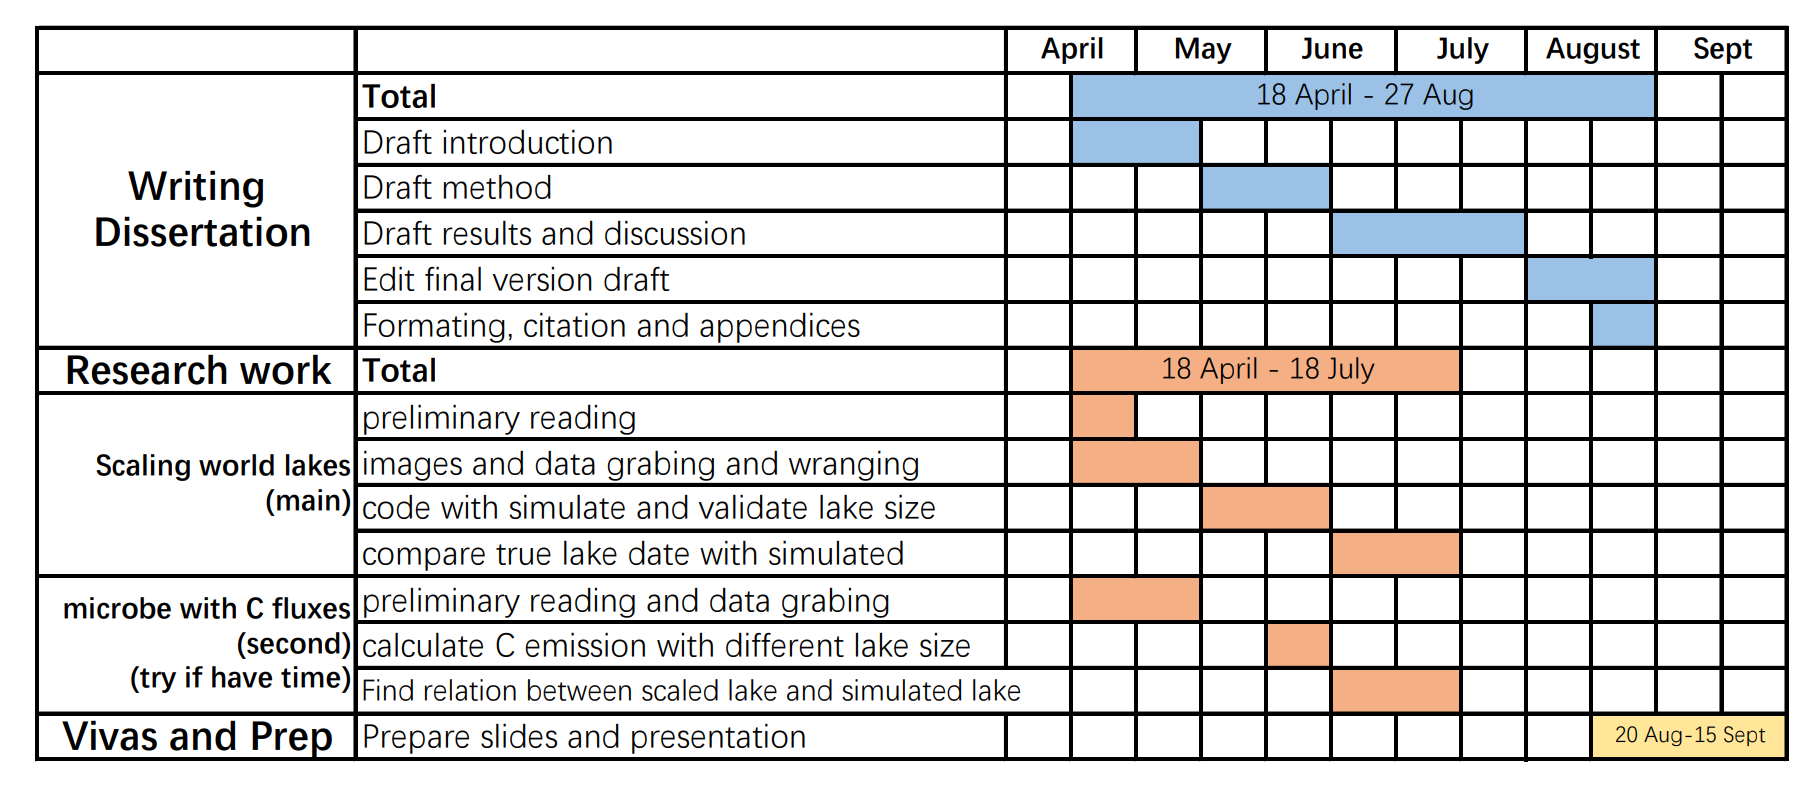
\includegraphics[scale=0.4]{introduction/Figure1.png}
    \caption{MSc Imperial Project}
    \label{Fig.1}
\end{figure}

\section{Budget}
Other items that might enhance project completion are presented in Figure 2. Each item is accompanied with a rationale of its use and an estimated of cost. 

\begin{figure}[H]
    \centering
    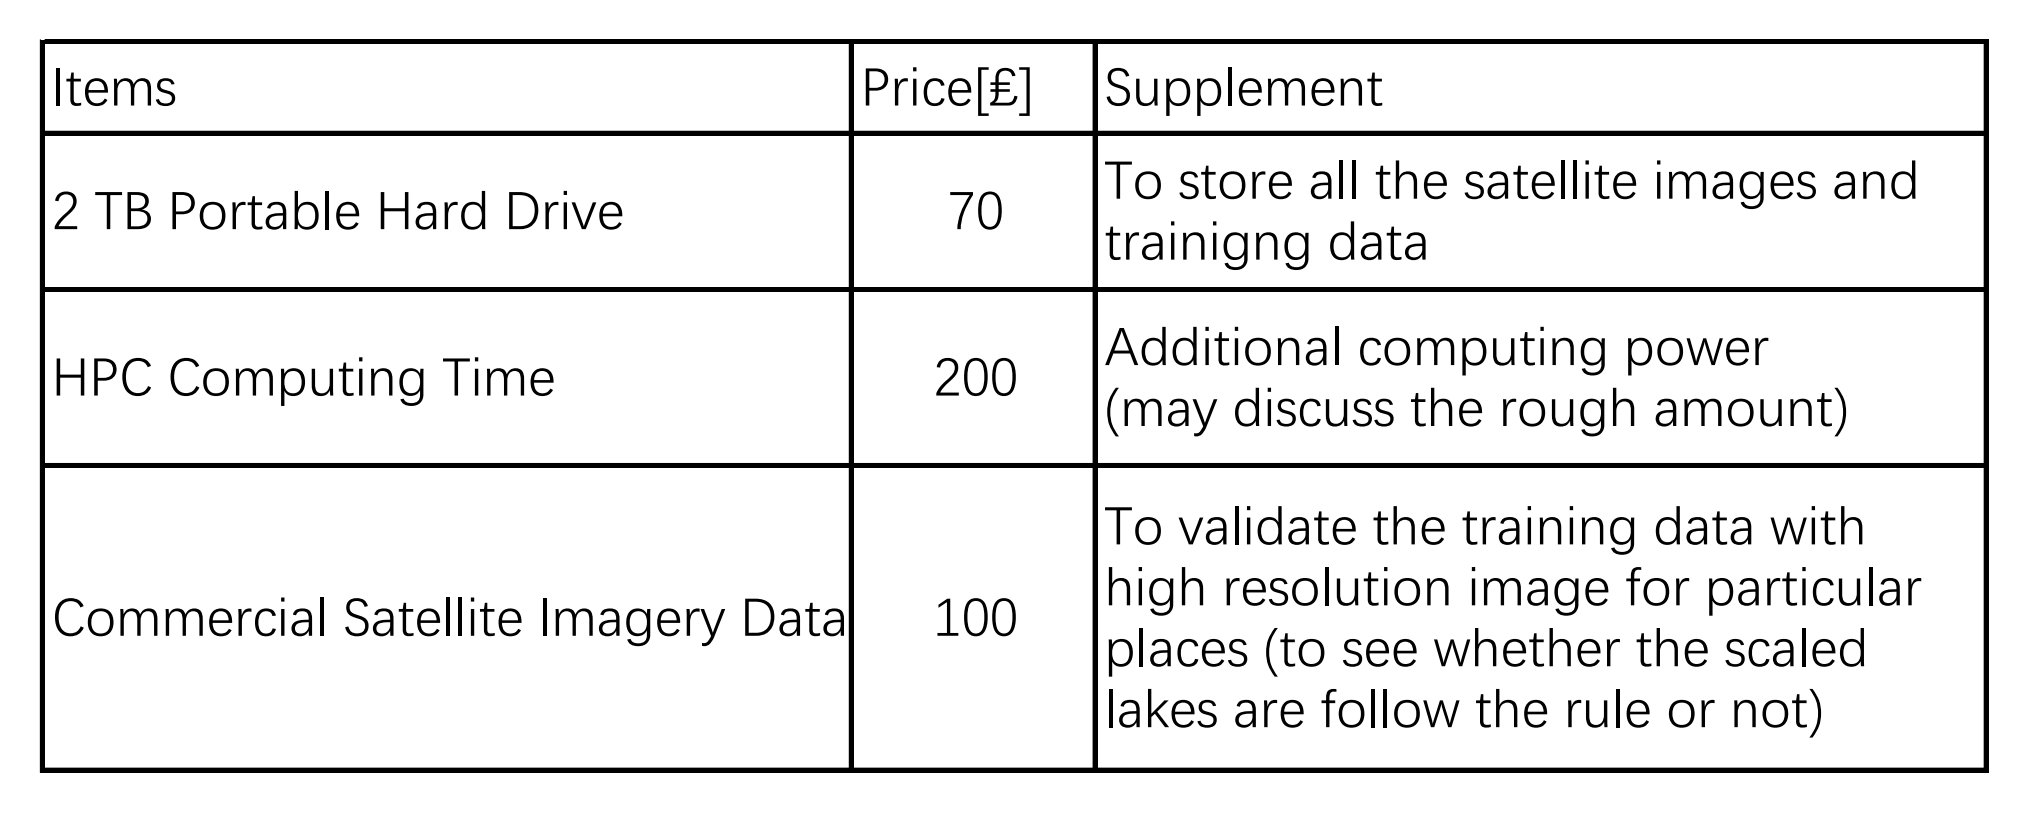
\includegraphics[scale=0.3]{introduction/Figure2.png}
    \caption{Budget}
    \label{Fig.2}
\end{figure}

\section{Supervisor Declaration}
\large{I have seen and approved the project and budget.}
\\
\large{Supervisor Signature:}     
\\
\large{Date:}

